\section{Ludwig 英文语句搜索引擎}%
\label{sec:writing-ludwig}

Ludwig 英文语句搜索引擎可以帮助研究者选择适用的词句。现在以一个标题为例:
Solving a Perishables Joint Pricing and Inventory Control Problem
with \ldots.
对于一个以英语为母语或者工作语言的人来看,这个标题是有点问题的。
对于不常用英文写作的研究者,也是情有可原。
为了提高英文写作水平,可以考虑使用
\href{https://ludwig.guru/}{ludwig.guru/} 来搜索文献中使用相关词汇的语句。

如果我们对 Perishables Joint Pricing and Inventory Control
不确定正确与否,可以在搜索框中查看英文文献中对这个短语的使用情况,参见图
\S\ref{fig:ludwig-search}。

\begin{figure}[!htbp]
  \centering
  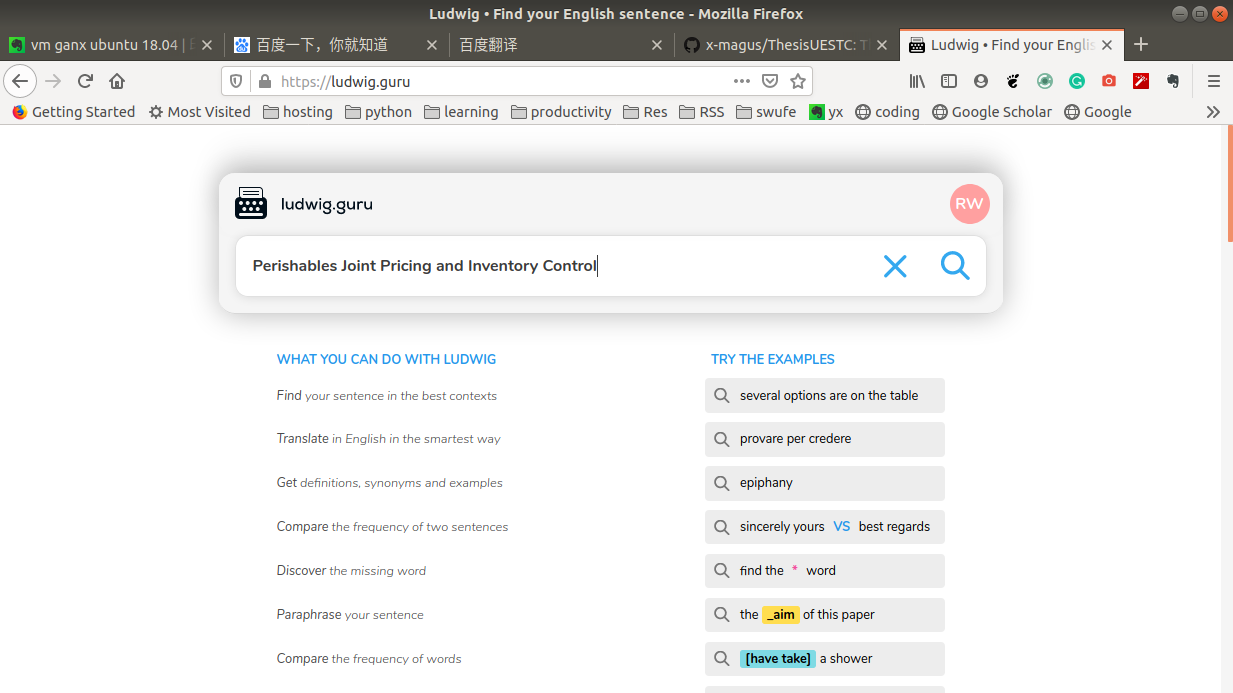
\includegraphics[width=1.0\textwidth]{media/shots/ludwig/Screenshot from 2019-12-23 21-13-03.png}
  \caption{搜索 Perishables Joint Pricing and Inventory Control}%
  \label{fig:ludwig-search}
\end{figure}

从图 \S\ref{fig:ludwig-result-1} 及 \S\ref{fig:ludwig-result-2}
可以看到,搜索的结果不理想。
因为 Ludwig 使用的语言资料库太大,搜索结果不理想时可以考虑缩小搜索范围。
注意到缺省情况下筛选功能是关闭了的(可以看到 filter OFF
字样),我们可以打开筛选选项,根据实际情况选择搜索范围。详情参见图
\S\ref{fig:ludwig-filter}.

令人遗憾的是,搜索结果任然不理想(见图
\S\ref{fig:ludwig-result-3}),没有看到完整的匹配,只看到左中位置显示的 60
SIMILAR 提示。
这时,我们可以考虑搜索更少的关键词。
从搜索结果中,我们发现 Perishables
和其它关键词甚少关联,可以考虑去掉这个关键词后重新搜索。
搜索结果见图 \S\ref{fig:ludwig-result-4},
我们可以看到仍然没有得到完美匹配,只看到 60 SIMILAR 提示。
但令人欣慰的是,在第一个结果中,我们看到了除大小写外的完美匹配。
可以理解成这个搜索是大小写敏感的。
这时我们可以考虑把搜索框中的大写字母全部改成小写字母来搜索。
搜索结果见图 \S\ref{fig:ludwig-result-5}, 我们可以看到两个完美匹配
(2 EXACT).

\begin{figure}[!htbp]
  \centering
  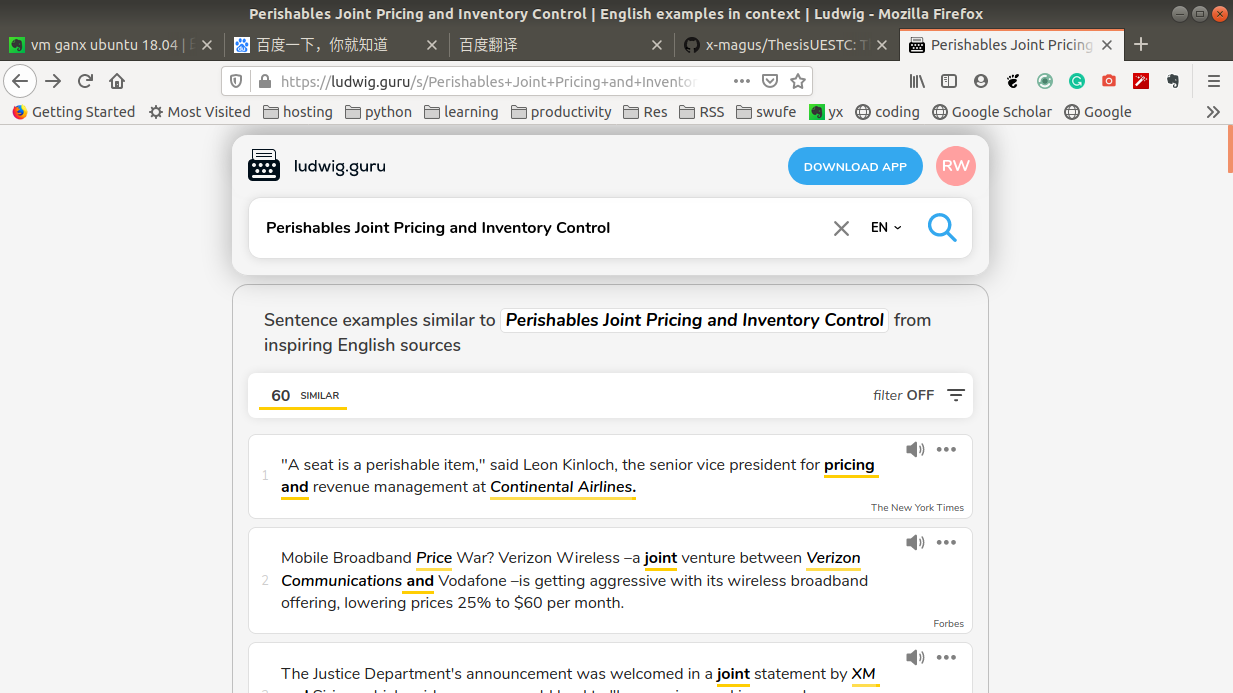
\includegraphics[width=1.0\textwidth]{media/shots/ludwig/Screenshot from 2019-12-23 21-16-43.png}
  \caption{搜索结果 1}%
  \label{fig:ludwig-result-1}
\end{figure}

\begin{figure}[!htbp]
  \centering
  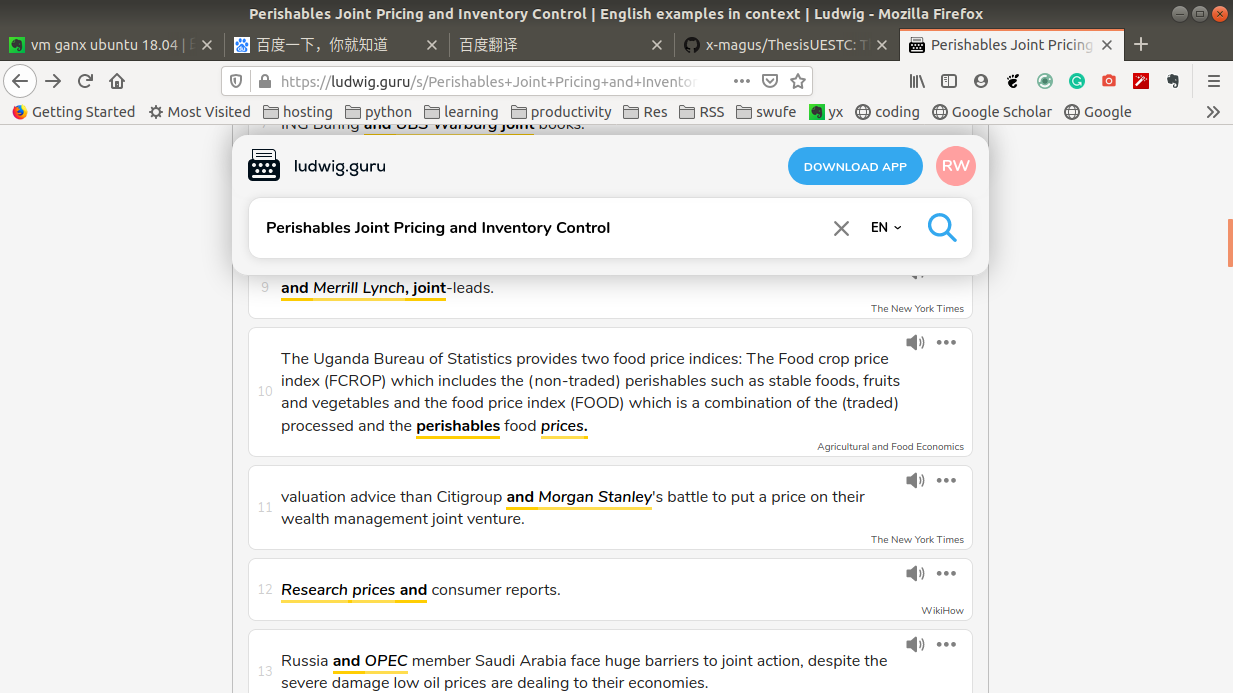
\includegraphics[width=1.0\textwidth]{media/shots/ludwig/Screenshot from 2019-12-23 21-16-55.png}
  \caption{搜索结果 2}%
  \label{fig:ludwig-result-2}
\end{figure}

\begin{figure}[!htbp]
  \centering
  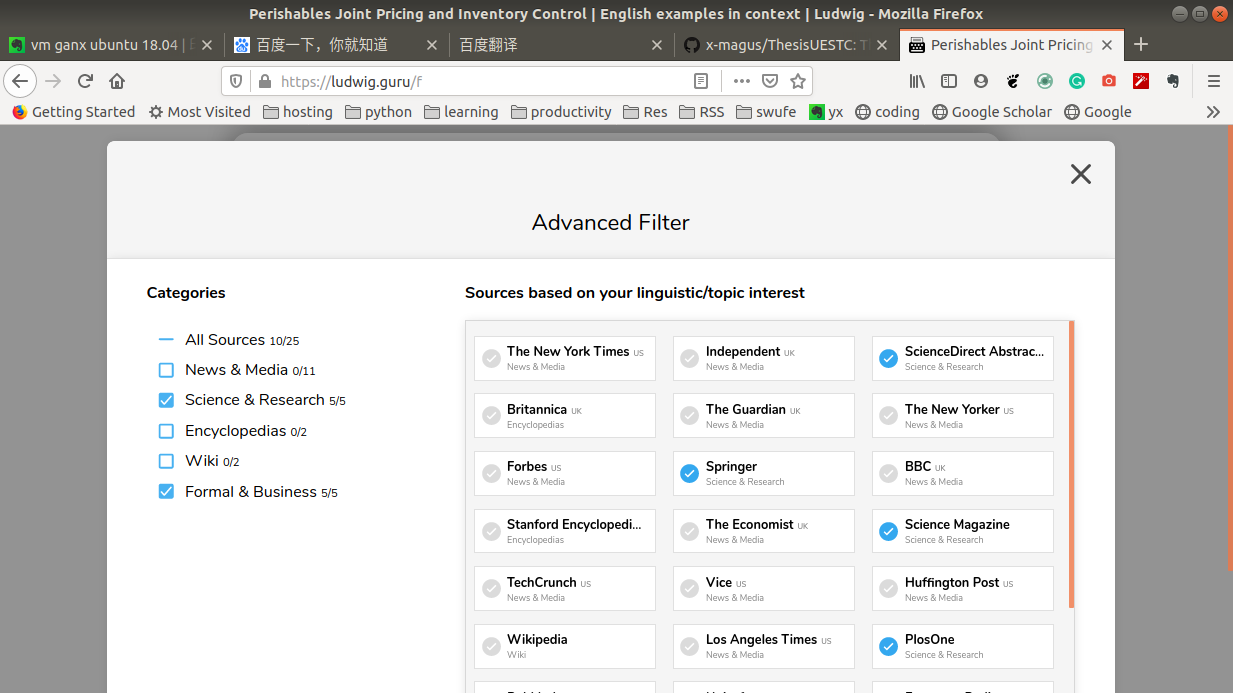
\includegraphics[width=1.0\textwidth]{media/shots/ludwig/Screenshot from 2019-12-23 21-17-32.png}
  \caption{筛选搜索范围}%
  \label{fig:ludwig-filter}
\end{figure}

\begin{figure}[!htbp]
  \centering
  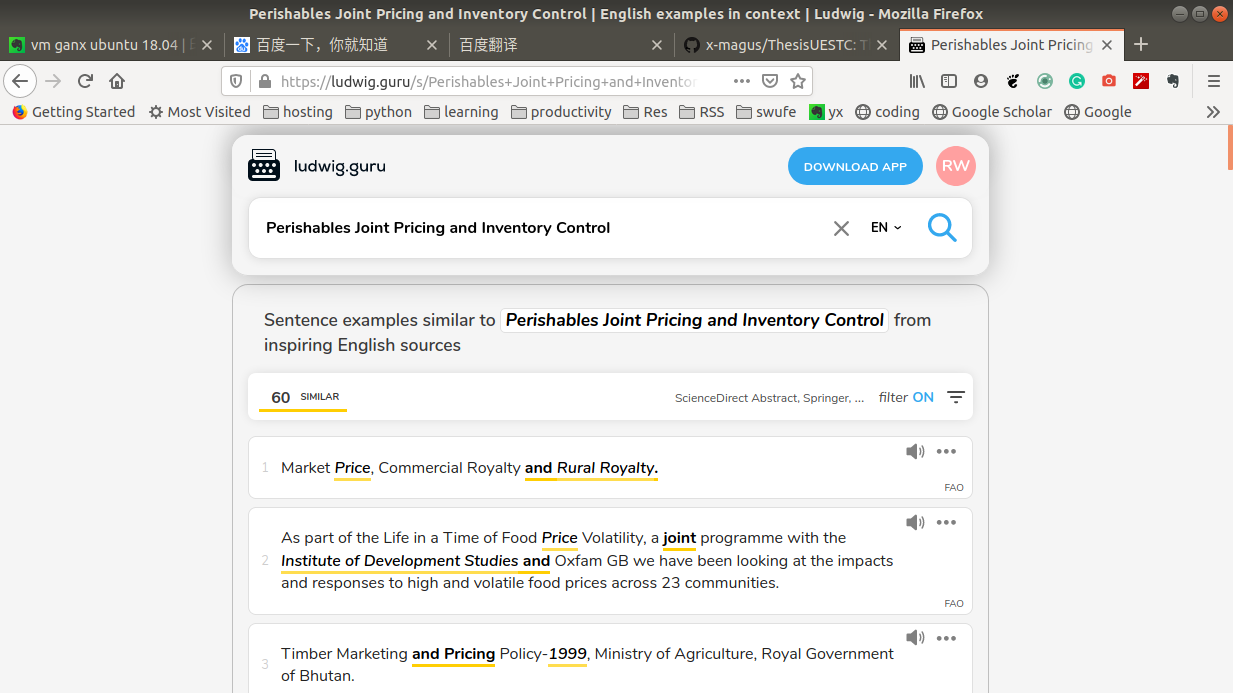
\includegraphics[width=1.0\textwidth]{media/shots/ludwig/Screenshot from 2019-12-23 21-18-09.png}
  \caption{搜索结果 3}%
  \label{fig:ludwig-result-3}
\end{figure}

\begin{figure}[!htbp]
  \centering
  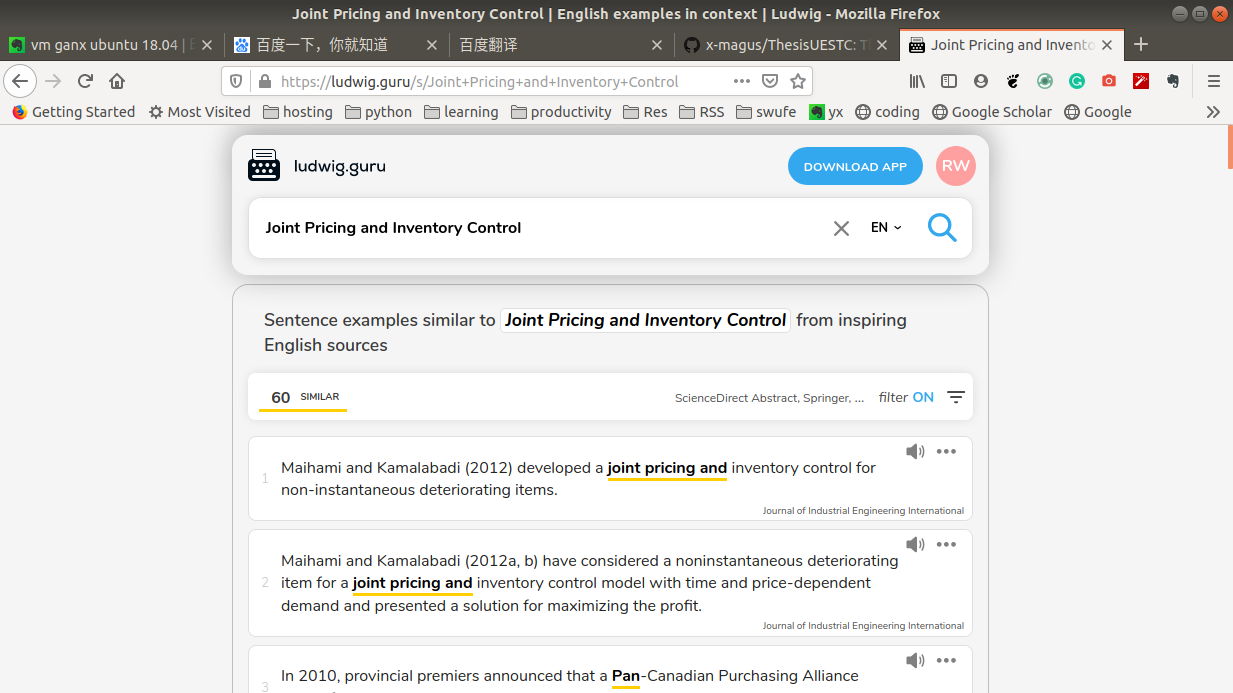
\includegraphics[width=1.0\textwidth]{media/shots/ludwig/Screenshot from 2019-12-23 21-19-22.png}
  \caption{去掉 Perashables 后的搜索结果}%
  \label{fig:ludwig-result-4}
\end{figure}

\begin{figure}[!htbp]
  \centering
  \includegraphics[width=1.0\textwidth]{media/shots/ludwig/Screenshot from
  2019-12-23 21-20-01.png}
  \caption{去掉 Perashables 后且使用小写字母的搜索结果}%
  \label{fig:ludwig-result-5}
\end{figure}

